\documentclass[conference]{IEEEtran}
\IEEEoverridecommandlockouts
% The preceding line is only needed to identify funding in the first footnote. If that is unneeded, please comment it out.
\usepackage{cite}
\usepackage{amsmath,amssymb,amsfonts}
\usepackage{algorithmic}
\usepackage{graphicx}
\usepackage{hyperref}
\usepackage{eso-pic}
\usepackage{enumitem}
\usepackage{makecell}
\usepackage{textcomp}
\usepackage{listings}
\usepackage{xcolor}
\def\BibTeX{{\rm B\kern-.05em{\sc i\kern-.025em b}\kern-.08em
    T\kern-.1667em\lower.7ex\hbox{E}\kern-.125emX}}
\begin{document}
\iffalse
\AddToShipoutPictureBG*{
  \AtPageUpperLeft{
    \hspace{1.5 cm} 
    \raisebox{-4.7 cm}[0pt][0pt]{
      
\includegraphics[width=3.5 cm]{figs/IITH.png}
    }
  }
}
\fi

\title{Voice Based UGV control}
\author{
    \IEEEauthorblockN{Gajjarapu Satyanarayana  and G.V.V. Sharma} 
    %\IEEEauthorblockN{Gautam Singh} 
    %\IEEEauthorblockA{EE Department, Indian Institute of Technology Hyderabad,\\
    %\and
    %\IEEEauthorblockN{Sachinkumar Omprakash Dubey} 
    %\and
    %\IEEEauthorblockN{G. V. V. Sharma} 
    %\and
    \IEEEauthorblockA{Department of Electrical Engineering, 
	    \\
	    Indian Institute of Technology Hyderabad,\\
    Kandi, India 502284
\\
gadepall@ee.iith.ac.in}
}

\maketitle

%\tableofcontents

\renewcommand{\thefigure}{\theenumi}
\renewcommand{\thetable}{\theenumi}

\bigskip

\begin{abstract}
In this paper, we demonstrate how to guide an unmanned ground vehicle (UGV) using a gamepad interface as well as voice commands. This is done through an android application for sensing voice or touch on the phone and  relaying the control data to the UGV via Bluetooth.  In the process, we show how this platform 
offers a low-cost alternative for porting artifical intelligence (AI) algorithms on hardware.  
\iffalse
driven study motor control, wireless communication by combining basic autonomous navigation.

The UGV is built using an ESP32 microcontroller and L293D motor driver IC to drive two DC motors. Users can control the toycar through a mobile app that provides a gamepad interface or takes voice commands. 
\fi
\end{abstract}

\section{Introduction}
Autonomous navigation has been a major area of research in robotics, with pioneering projects such as Stanley, which won the DARPA Grand Challenge \cite{thrun2006stanley}, and Boss and Junior, which competed in the DARPA Urban Challenge \cite{urmson2008boss, montemerlo2008junior}, demonstrating autonomous navigation in complex environments. End-to-end learning approaches, such as NVIDIA's system for self-driving cars \cite{bojarski2016end}, have further simplified navigation pipelines by mapping sensor inputs directly to control outputs. Surveys on intelligent vehicles highlight a wide variety of autonomous driving applications \cite{bishop2000survey}, and research on fully autonomous systems explores both the hardware and software required for robust navigation \cite{levinson2011towards}. In parallel, speech-based human-robot interaction has enabled intuitive control of robots in constrained environments, including intelligent wheelchairs and mobile robots \cite{li2017speech, prasad2013voice, vasudevan2010speech}, and robust speech recognition datasets such as Google’s Speech Commands \cite{warden2018speech} have accelerated development of voice-controlled systems. Inspired by these high-level projects, this work presents a scaled-down prototype using an ESP32 microcontroller and an L293D motor driver IC to build a voice-enabled toy car, integrating simple navigation with bluetooth control and speech commands for user interaction.

\section{List of Components}
\begin{enumerate}[label=\thesection.\arabic*,ref=\thesection.\theenumi]
\item The components used in this project and their description are listed in the Table \ref{table:list}
\begin{table}[h!]
  \centering
  \begin{tabular}[12pt]{ |c| c| c|}
    \hline
    \textbf{Item} & \textbf{Qty.} & \textbf{Description} \\ 
    \hline
    UGV kit & 1 & For assembling the toycar chassis.\\ 
    \hline
    ESP32 & 1 & \makecell{Microcontroller used for control \\ and wireless communication.} \\
    \hline
    L293D Motor Driver IC & 1 & For driving and controlling the DC motors. \\ 
    \hline
    Power Bank & 1 & Provides portable power supply to the system. \\
    \hline
    DC Motors & 2 & Used for propulsion of the toy car. \\
    \hline
    Breadboard & 1 & For making circuit connections. \\
    \hline
    Jumper Wires & 11 & \makecell{For making electrical connections \\ between components.} \\
    \hline
    Micro-USB cable & 1 & \makecell{Connection between the ESP32 \\ and the power bank.} \\
    \hline
    \end{tabular}


  \caption{List of Components}
  \label{table:list}
\end{table}

\end{enumerate}

\section{Hardware Setup}
%
\begin{enumerate}[label=\thesection.\arabic*,ref=\thesection.\theenumi]

\item Assemble the chassis, fix the motors and mount the wheels to build the toycar.

\item Fix the breadboard on the base of the toycar.

\item Plug the \textbf{L293D} motor driver IC in Fig. \ref{fig:l293d_ic} on the breadboard.

\begin{figure}[!ht]
\centering
\resizebox{0.4\textwidth}{!}{%
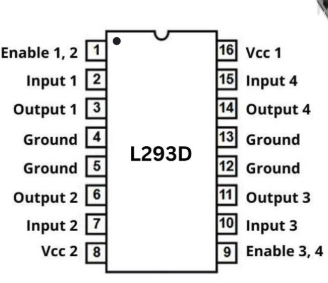
\includegraphics{figs/L293D_IC.png}
}%
\caption{L293D Motor Driver IC}
\label{fig:l293d_ic}
\end{figure}

\item The connections between the L293D output pins and the motors ($M_1, M_2$) are according to Table \ref{table:1}
\begin{table}[h!]
  \centering
  \begin{tabular}[12pt]{ |c| c| c| c| c|}
    \hline
    \textbf{L293D IC} & 3 & 6 & 11 & 14 \\ 
    \hline
    \textbf{Motors} & $M_1$ (+) & $M_1$ (-) & $M_2$ (+) & $M_2$ (-)\\ 
    \hline 
    \end{tabular}

  \caption{L293D \& Motors connections}
  \label{table:1}
\end{table}

\item Connect any 4 GPIO pins (\textbf{Ex}: 25, 26, 33 \& 32) of \textbf{ESP32} in Fig. \ref{fig:esp32} to L293D inputs
\begin{figure}[!ht]
\centering
\resizebox{0.4\textwidth}{!}{%
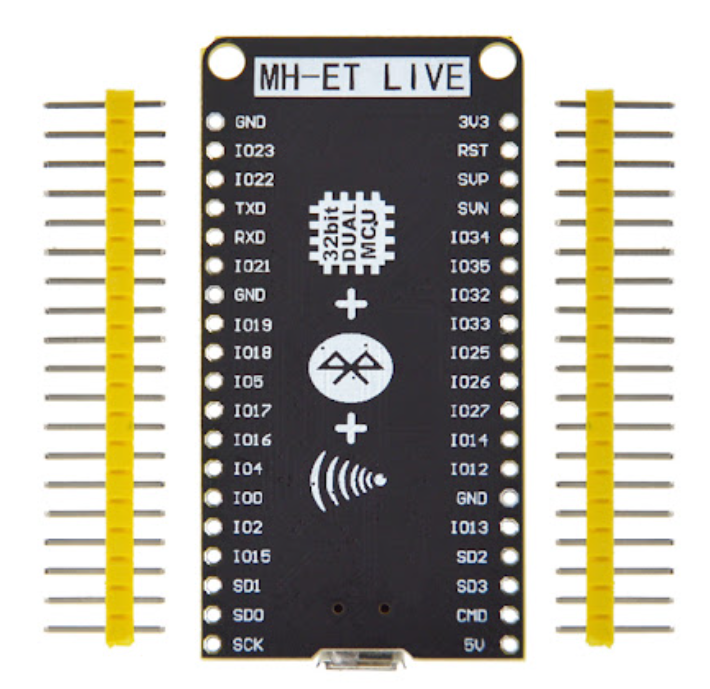
\includegraphics{figs/ESP32.png}
}%
\caption{ESP 32}
\label{fig:esp32}
\end{figure}
\item The connections between the ESP32 and the L293D input pins are according to Table \ref{table:2}
\begin{table}[h!]
  \centering
  \begin{tabular}[12pt]{ |c| c| c| c| c|}
    \hline
    \textbf{ESP32} & 32 & 33 & 25 & 26 \\ 
    \hline
    \textbf{L293D IC} & 3 & 6 & 11 & 14 \\ 
    \hline
    \end{tabular}

  \caption{L293D \& ESP32 connections}
  \label{table:2}
\end{table}

\item Connect the ground pins of the L293D IC and the ESP32 to a common ground on the breadboard.  

\item Connect the 5V pin of the ESP32 to the VCC 1 pin of the L293D IC.  

\end{enumerate}
%
\section{Implementation}

\subsection{Dabble}
\begin{enumerate}[label=\thesection.\arabic*
,ref=\thesection.\theenumi]

\item Install \textbf{Dabble} app using Google Playstore in an Android mobile.

\item Upload the following code to the ESP32 using any IDE.
\fbox{\parbox{\linewidth}{%
wget \url{https://github.com/Satyanarayana-123456/UGV_toycar/blob/main/codes/dabble_gamepad.cpp}%
}}

\item After uploading the above code, plug the ESP32 to a power bank via a micro-USB cable.

\item Open the Dabble app and connect to the ESP32 via bluetooth. The app interface looks like Fig. \ref{fig:dabble_home}
\begin{figure}[!ht]
\centering
\resizebox{0.4\textwidth}{!}{%
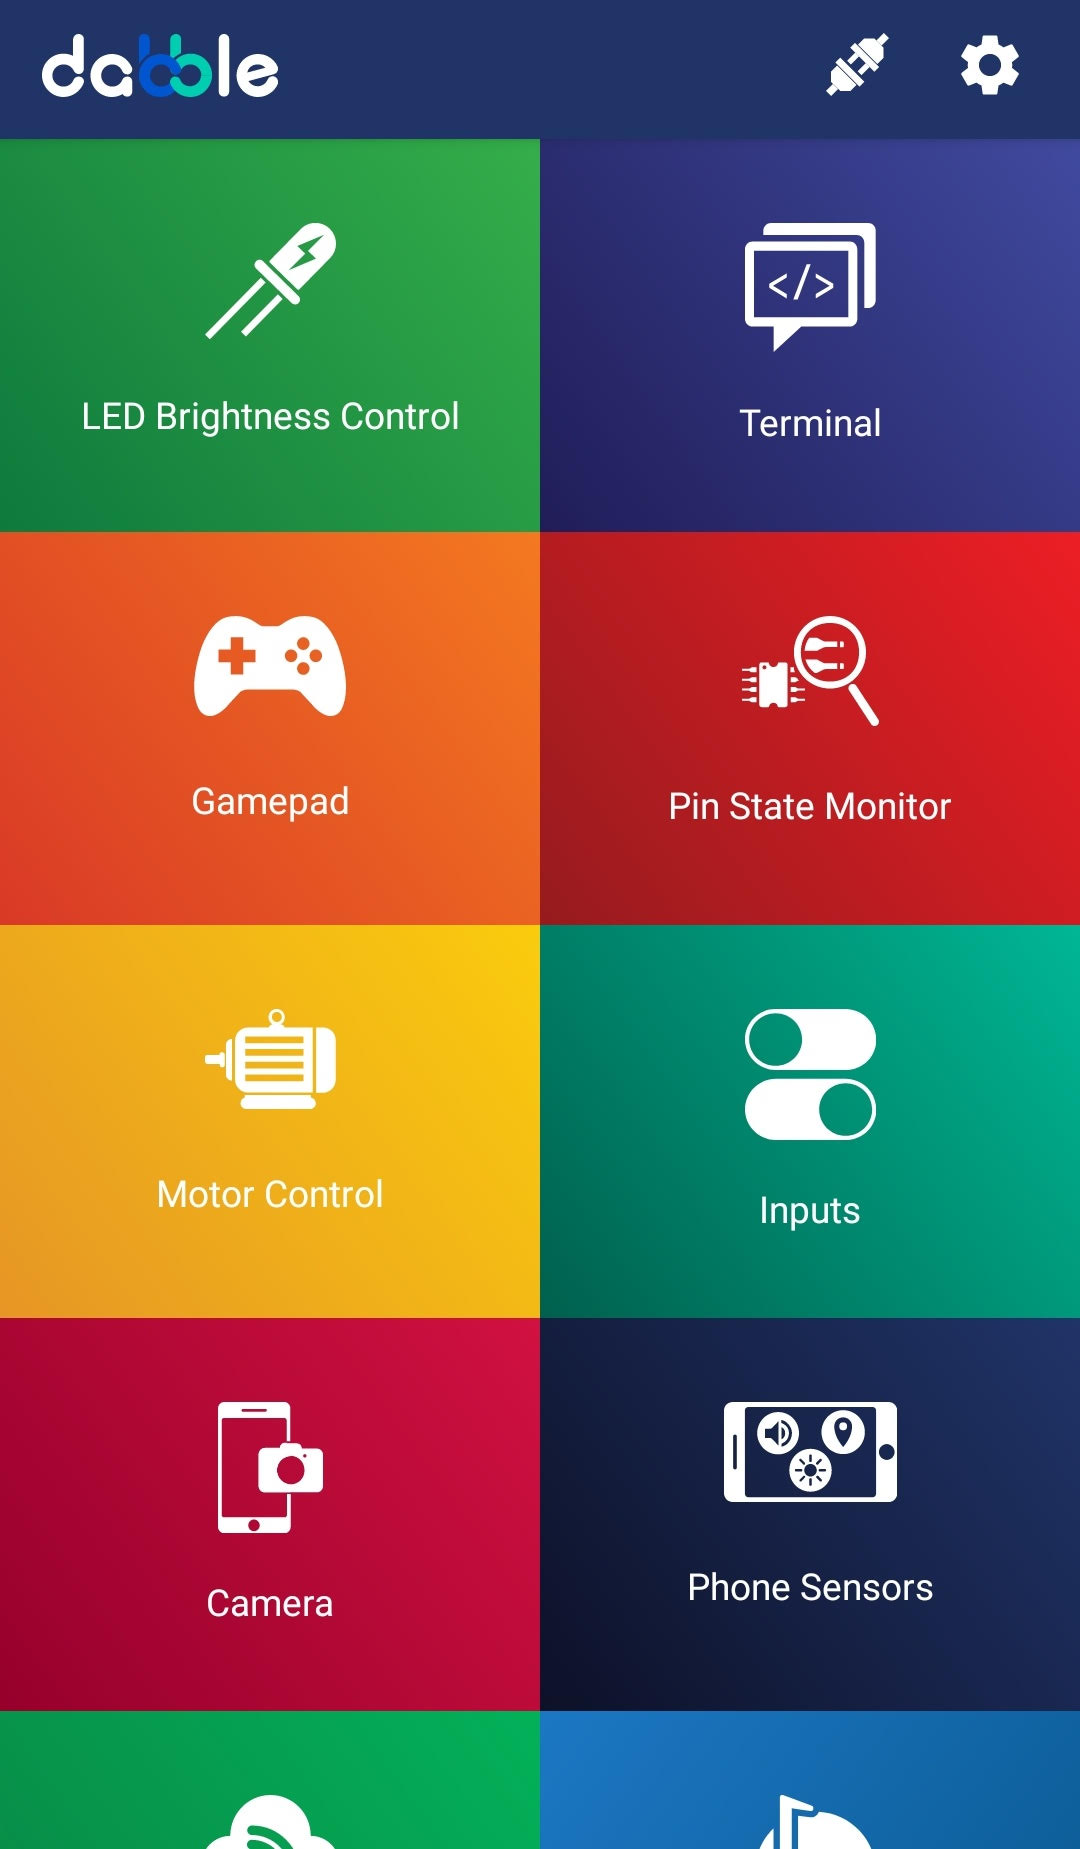
\includegraphics{figs/dabble_home.jpg}
}%
\caption{Dabble Interface}
\label{fig:dabble_home}
\end{figure}

\item Now use the \textbf{Gamepad} of the app in Fig. \ref{fig:dabble_gamepad} to control the toycar.
\begin{figure}[!ht]
\centering
\resizebox{0.5\textwidth}{!}{%
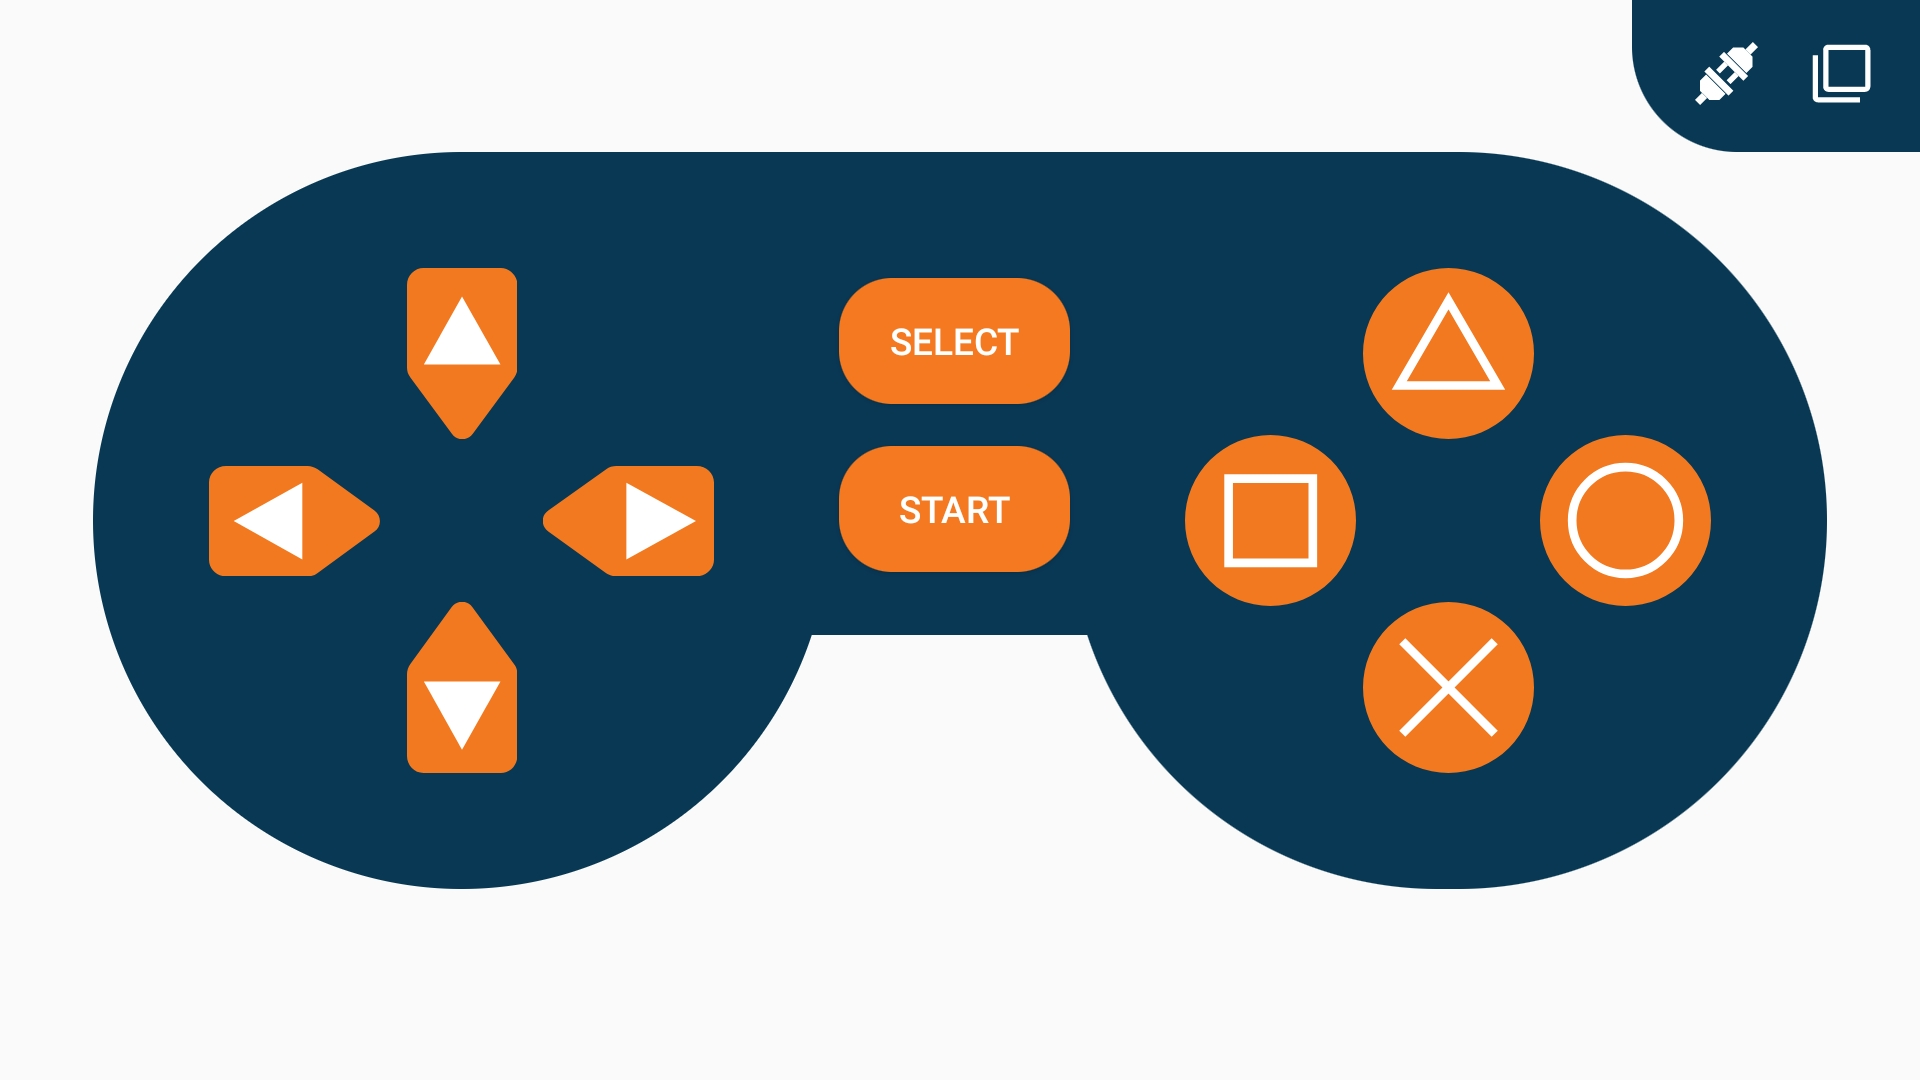
\includegraphics{figs/dabble_gamepad.jpg}
}%
\caption{Gamepad in Dabble App}
\label{fig:dabble_gamepad}
\end{figure}

\item Operate the left-side control buttons labeled \textit{Forward, Back, Left \& Right} to give the respective commands.

\subsection{Arduino Bluetooth Controller}

\item Install \textbf{Arduino Bluetooth Controller} app using Google Playstore in an Android mobile.

\item Upload the following code to the ESP32 using any IDE.
\fbox{\parbox{\linewidth}{%
wget \url{https://github.com/Satyanarayana-123456/UGV_toycar/blob/main/codes/ABC_voice.cpp}%
}}

\item After uploading the above code, plug the ESP32 to a power bank via a micro-USB cable.

\item Open the Arduino Bluetoth Controller app and connect to the ESP32 via bluetooth. The app interface looks like Fig. \ref{fig:ABC_home}

\begin{figure}[!ht]
\centering
\resizebox{0.4\textwidth}{!}{%
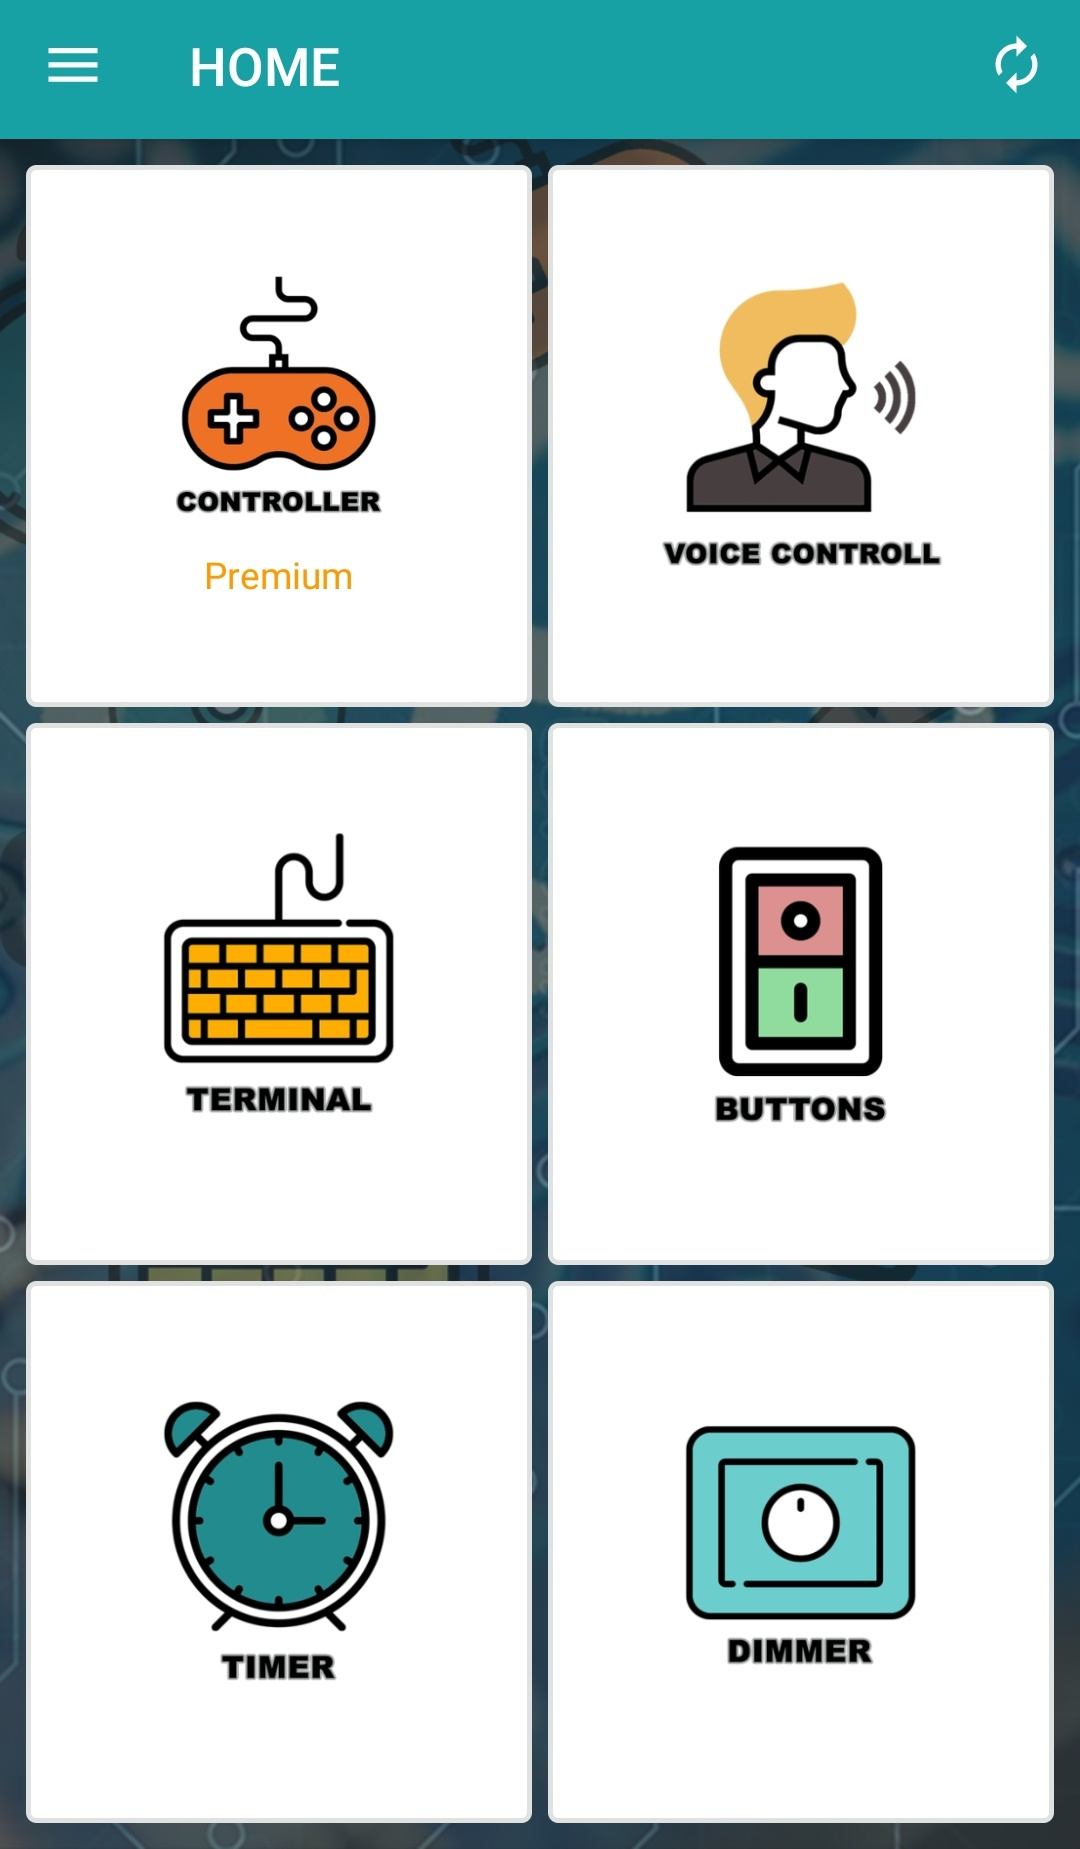
\includegraphics{figs/ABC_home.jpg}
}%
\caption{Arduino Bueetoth Controller Interface}
\label{fig:ABC_home}
\end{figure}

\item Now use the \textbf{Voice Control} section of the app to control the toycar.

\item The commands which the voice control takes are \textit{Left, Right, Forward, Back \& Stop}.

\end{enumerate}
\begin{thebibliography}{00}

\bibitem{thrun2006stanley}
S. Thrun et al., ``Stanley: The robot that won the DARPA Grand Challenge,'' \textit{Journal of Field Robotics}, vol. 23, no. 9, pp. 661–692, 2006.

\bibitem{urmson2008boss}
C. Urmson et al., ``Autonomous driving in urban environments: Boss and the Urban Challenge,'' \textit{Journal of Field Robotics}, vol. 25, no. 8, pp. 425–466, 2008.

\bibitem{montemerlo2008junior}
M. Montemerlo et al., ``Junior: The Stanford entry in the Urban Challenge,'' \textit{Journal of Field Robotics}, vol. 25, no. 9, pp. 569–597, 2008.

\bibitem{bojarski2016end}
M. Bojarski et al., ``End to end learning for self-driving cars,'' \textit{arXiv preprint arXiv:1604.07316}, 2016. [Online]. Available: \url{https://arxiv.org/abs/1604.07316}

\bibitem{bishop2000survey}
R. Bishop, ``A survey of intelligent vehicle applications worldwide,'' \textit{IEEE Intelligent Vehicles Symposium}, vol. 15, no. 1, pp. 113–122, 2000.

\bibitem{levinson2011towards}
J. Levinson, J. Askeland, J. Becker et al., ``Towards fully autonomous driving: Systems and algorithms,'' in \textit{Proc. IEEE Intelligent Vehicles Symposium}, 2011, pp. 163–168.

\bibitem{li2017speech}
G. Li, S. Mei, H. Yang et al., ``Speech interaction with robots: A review,'' \textit{International Journal of Advanced Robotic Systems}, vol. 14, no. 6, pp. 1–15, 2017.

\bibitem{prasad2013voice}
P. R. K. Prasad, V. G. Kumar, and R. R. Reddy, ``Voice-controlled robotic vehicle,'' \textit{International Journal of Advanced Research in Electrical, Electronics and Instrumentation Engineering}, vol. 2, no. 6, pp. 2723–2728, 2013.

\bibitem{warden2018speech}
P. Warden, ``Speech commands: A dataset for limited-vocabulary speech recognition,'' \textit{arXiv preprint arXiv:1804.03209}, 2018.

\bibitem{vasudevan2010speech}
A. Vasudevan and R. Siegwart, ``Speech-based human–robot interaction for assistive robots,'' \textit{Robotics and Autonomous Systems}, vol. 58, no. 7, pp. 881–888, 2010.

\end{thebibliography}
\end{document}

